\documentclass[11pt]{article}
\renewcommand{\baselinestretch}{1.8}
\usepackage{textcomp}
\usepackage{fontenc}
\usepackage{graphicx}
\usepackage{caption} % for Fig. captions
\usepackage{gensymb} % for \degree
\usepackage{placeins} % for \images
\usepackage[margin=1in]{geometry} % to set margins
\usepackage{setspace}
\usepackage{lineno}
%\usepackage{cite}
\usepackage{amssymb} % for math symbols
\usepackage{amsmath} % for aligning equations
\usepackage{natbib}
\begin{document}
\section*{Background}
There is a general consensus that spring phenology of temperate woody plants is primary cued by forcing, chilling and photoperiod. Yet we (and a number of other studies) find that species differ in their cue use. We now seek to identify the evolutionary and ecological factors that may drive these differences.\\

As a lab we have come up with a few hypotheses--- Phylogenetic relationships, niches (personified by functional traits), and,what we focus on in this project, the environmental conditions that a species encounters in it native range shape it's cue use. In fact, a number of papers assume range differences among species drive differences phenological cue use, but as far as we can tell this hypothesis has not been rigorously tested.\\

Now, armed with species-level estimates of cue-use from our OSPREE database, grided climate data and species distribution maps, our team will range for to test this prediction.\\ 

\section*{Predictions}
From the literature, we arrive at a rather general prediction. If forcing (considered to be the primary cue) is an unreliable indicator of appropriate spring growing conditions, than species will rely more heavily on secondary cues. We also would expect that species must encounter the cue conditions (ie tropical species shouldn't have a chilling cue).\\

But what makes forcing unreliable? High inter and/ or intra-annual variability among locations or years. We think that the latter is more important, but a recent study boy Zohner found the former to matter.\\ 

Further, there is a general expectation that range size should positively correlated with environmental variability, and because climate patterns in Europe and North America are quite different, we would expect to see differences in cue use. We detail each hypothesis below.\\

\section*{Side bar: temporal vs. geographic variability}
When we talk about climate variability across a species' range, there are at least 2 axes which could be measured. Inter-annual variability for a given grid cell, or variation among grid cells at a give time. We think that both kinds of variation could in theory drive selection for cue use if we assume cue use is relatively conserved within species. It would be nice if these two axes were highly correlated, and it appears they sort of are for mean climate (not shown) but less so (Fig. \ref{fig:tempgeo}). We will decide how to treat this later, but for now we run models on both kinds of variation.


\section*{Hypotheses}
\subsection{Hypothesis 1: North America species (which experience a more variable spring environment) should have stronger photoperiod and chilling cue than European species.}
Seems to be supported by our data (Fig. \ref{fig:continent}).


\subsection{Hypothesis 2: Standard deviation of growing degree days until last frost should correlate with higher (more negative) chill sensitivity}. 
This hypothesis does not seem well supported by our data (Fig. \ref{fig:gddlf}).



\subsection{Hypothesis 3: Standard deviation of mean winter temperatures (STV) should correlate with higher (more negative) chill sensitivity}. 
This hypothesis was supported by Zohner's work. However, we think it might be an artifact of not explicitly including phenology into our models. Its also not supper supported in our data (Fig. \ref{fig:stv}).


\subsection{Hypothesis 4: Range margins drive chill or photoperiod sensitivity.}
See Fig. \ref{fig:lat}.

\section*{Alternative hypotheses}
We don't see a lot of support for our hypothesis. Here are  some other ideas we are thinking of testing.
\begin{enumerate}
\item Intra-specific variation in cue use is high.
\item How much overlap there is in species' ranges drive cue use difference
\end{enumerate}
\pagebreak[4]

\section*{Figures}
\begin{figure}[h!]
    \centering
         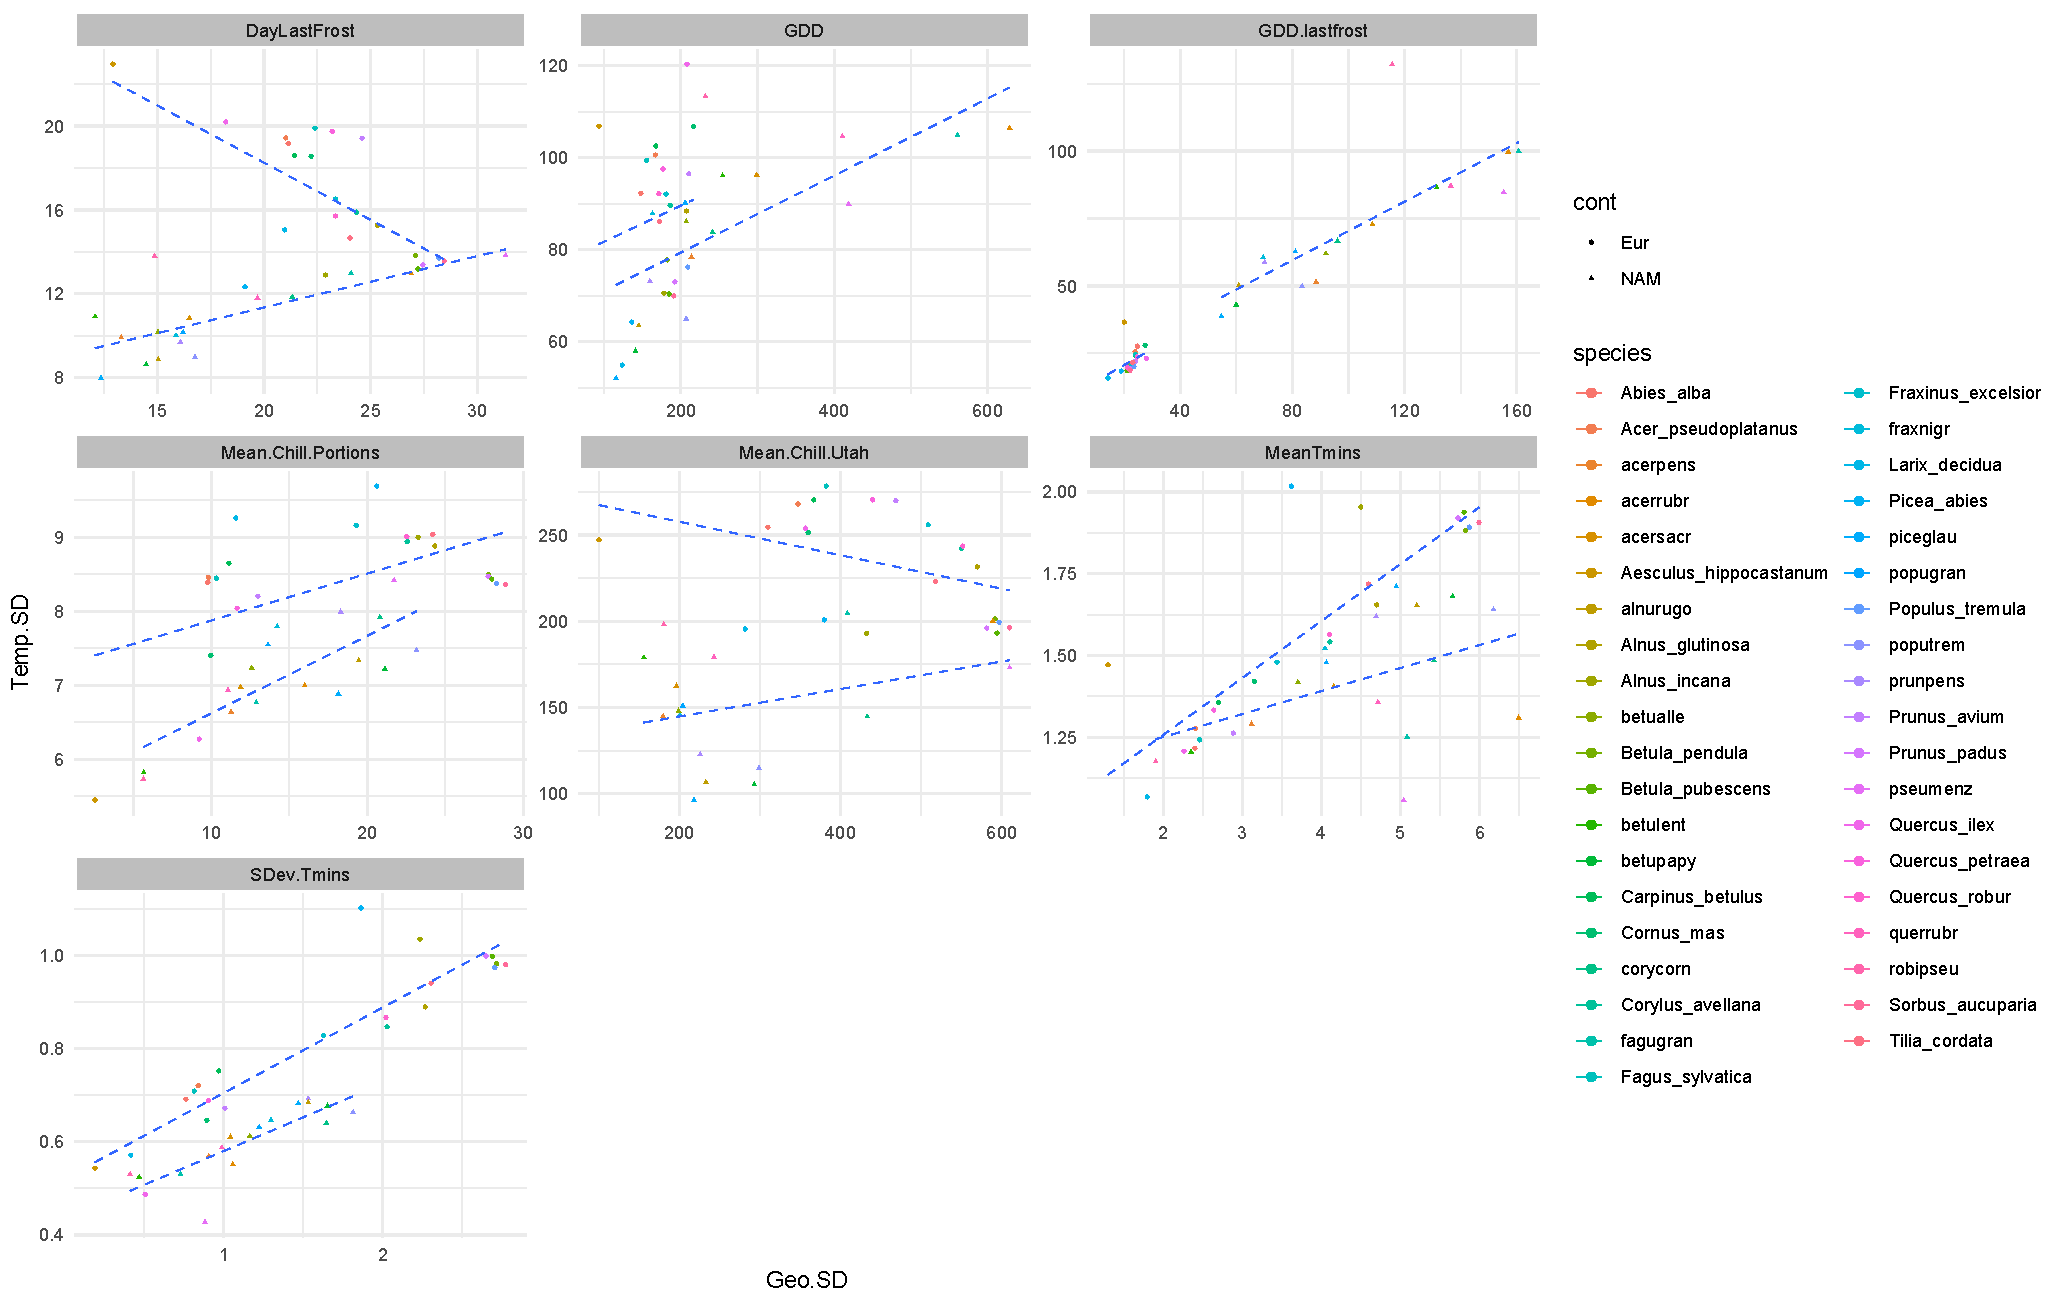
\includegraphics[width=.9\textwidth]{..//figures/spatial_vs_temporal/spatialtemporal_sds.pdf}
    \caption{Correlation between temporal and geographic standard deviation of climate parameters} 
    \label{fig:tempgeo}
\end{figure}

\begin{figure}[h!]
    \centering
         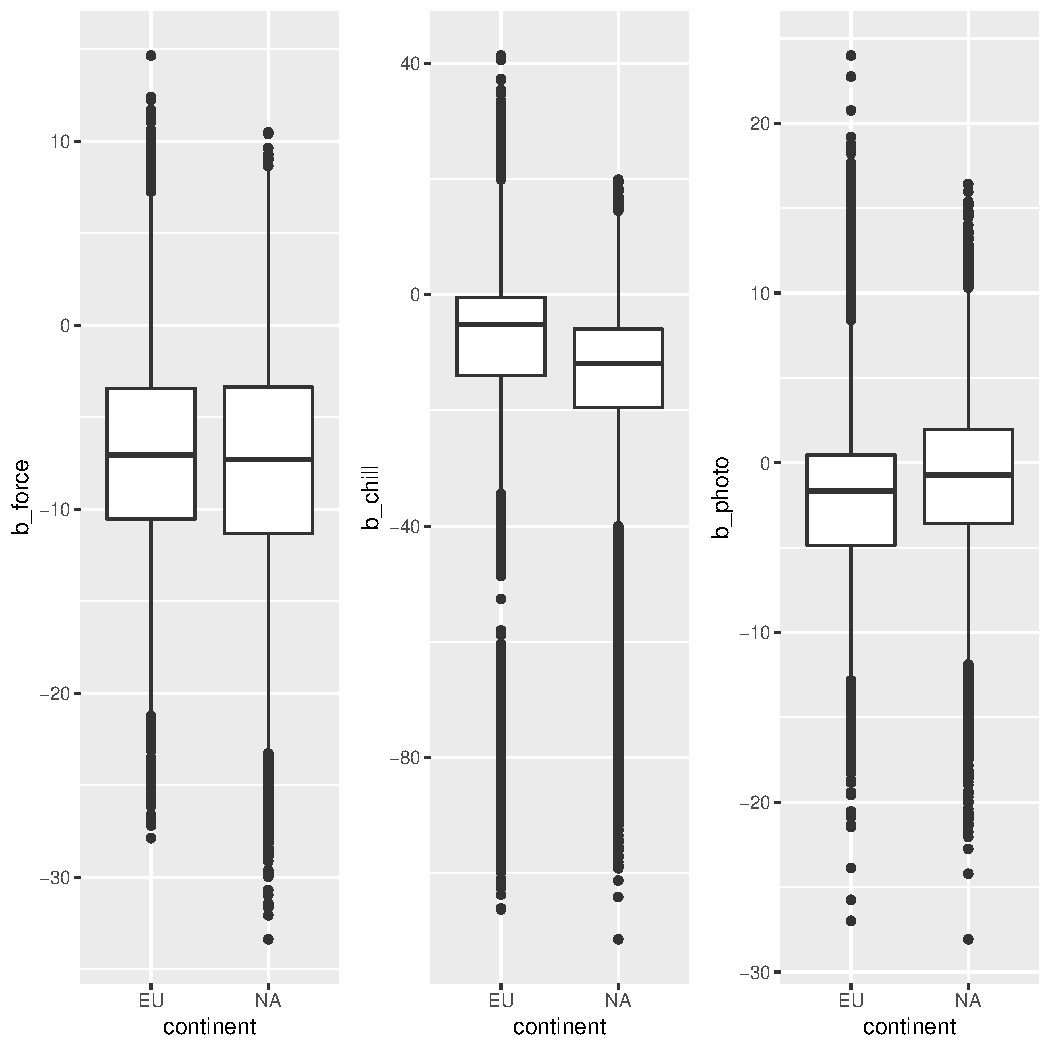
\includegraphics[width=.7\textwidth]{..//figures/continental_cues.pdf}
    \caption{ Chilling and Photoperiod cues use is stronger (more negative) in North America} 
    \label{fig:continent}
\end{figure}

\begin{figure}[h!]
    \centering
         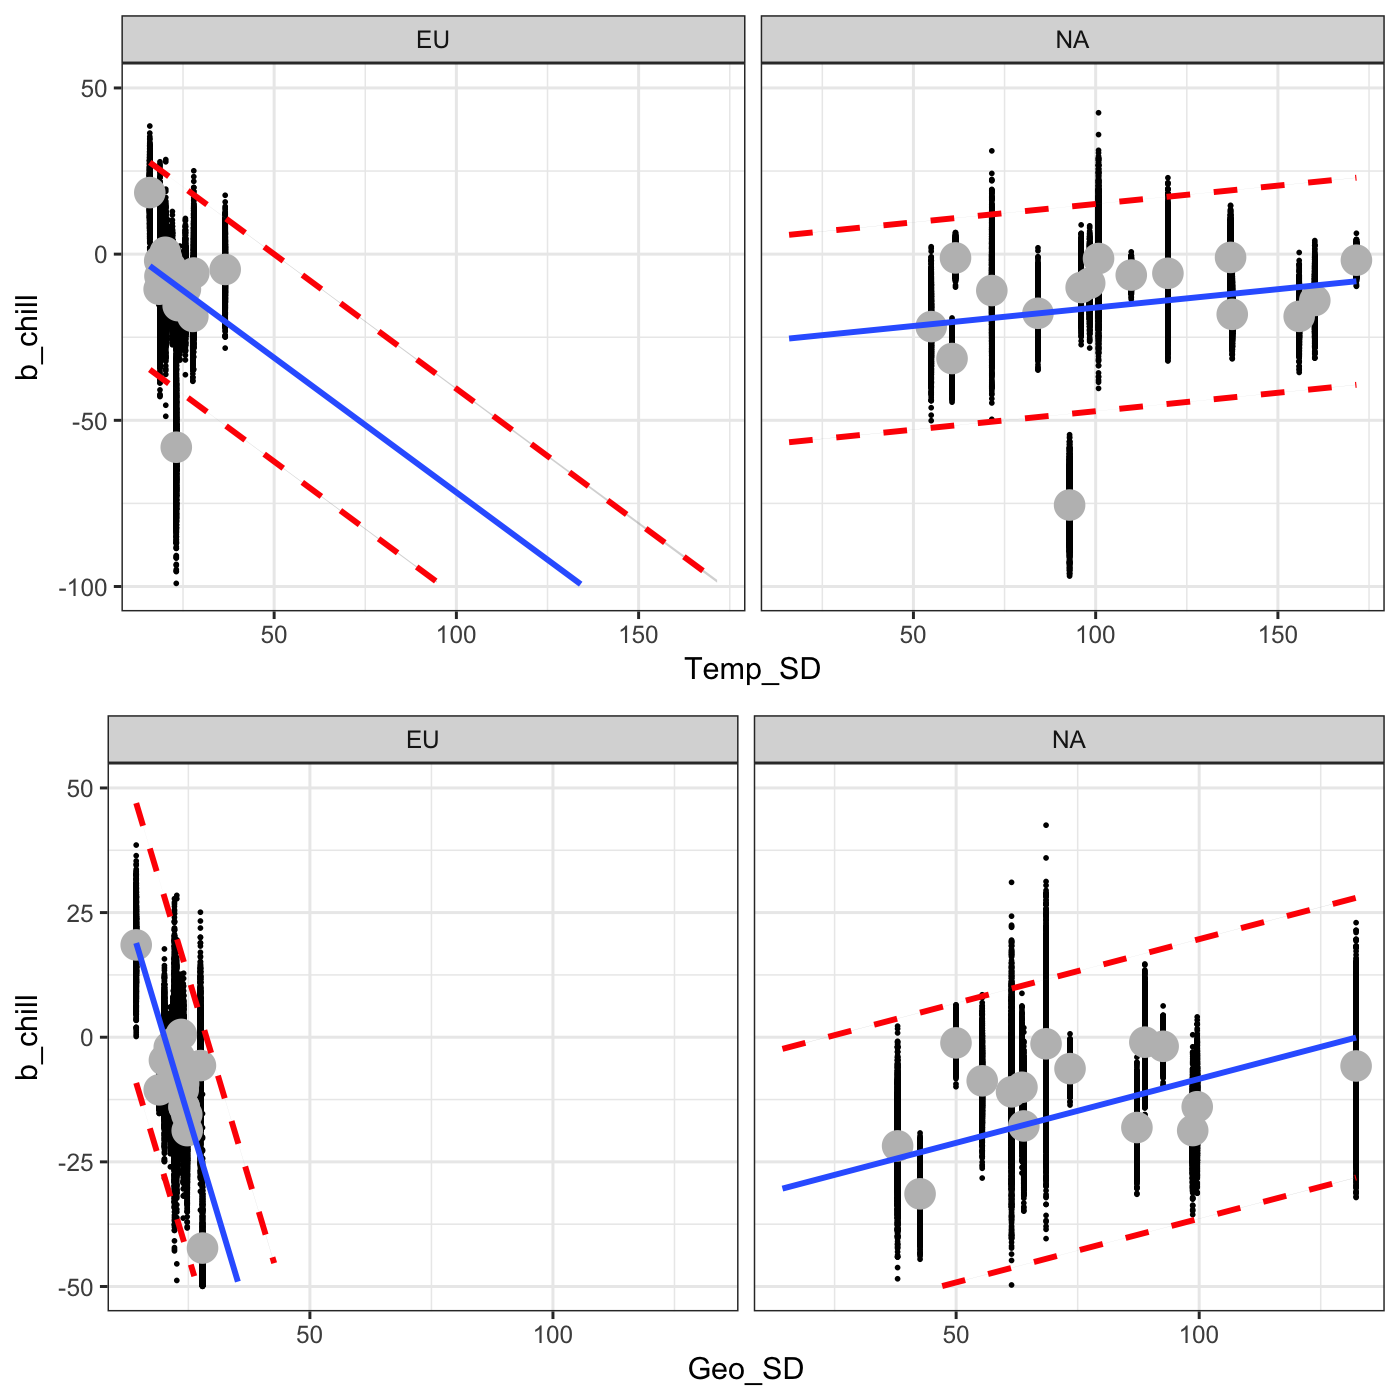
\includegraphics[width=.9\textwidth]{..//figures/cheap_approach/modeled_gdd2lf.png}
    \caption{Influence of temporal and geographic variation in growing degrees to last frost on $\beta_{chill}$. Model is pooling on iterations. Blue line is mean and red lines 95\% credible intervals} 
    \label{fig:gddlf}
\end{figure}


\begin{figure}[h!]
    \centering
         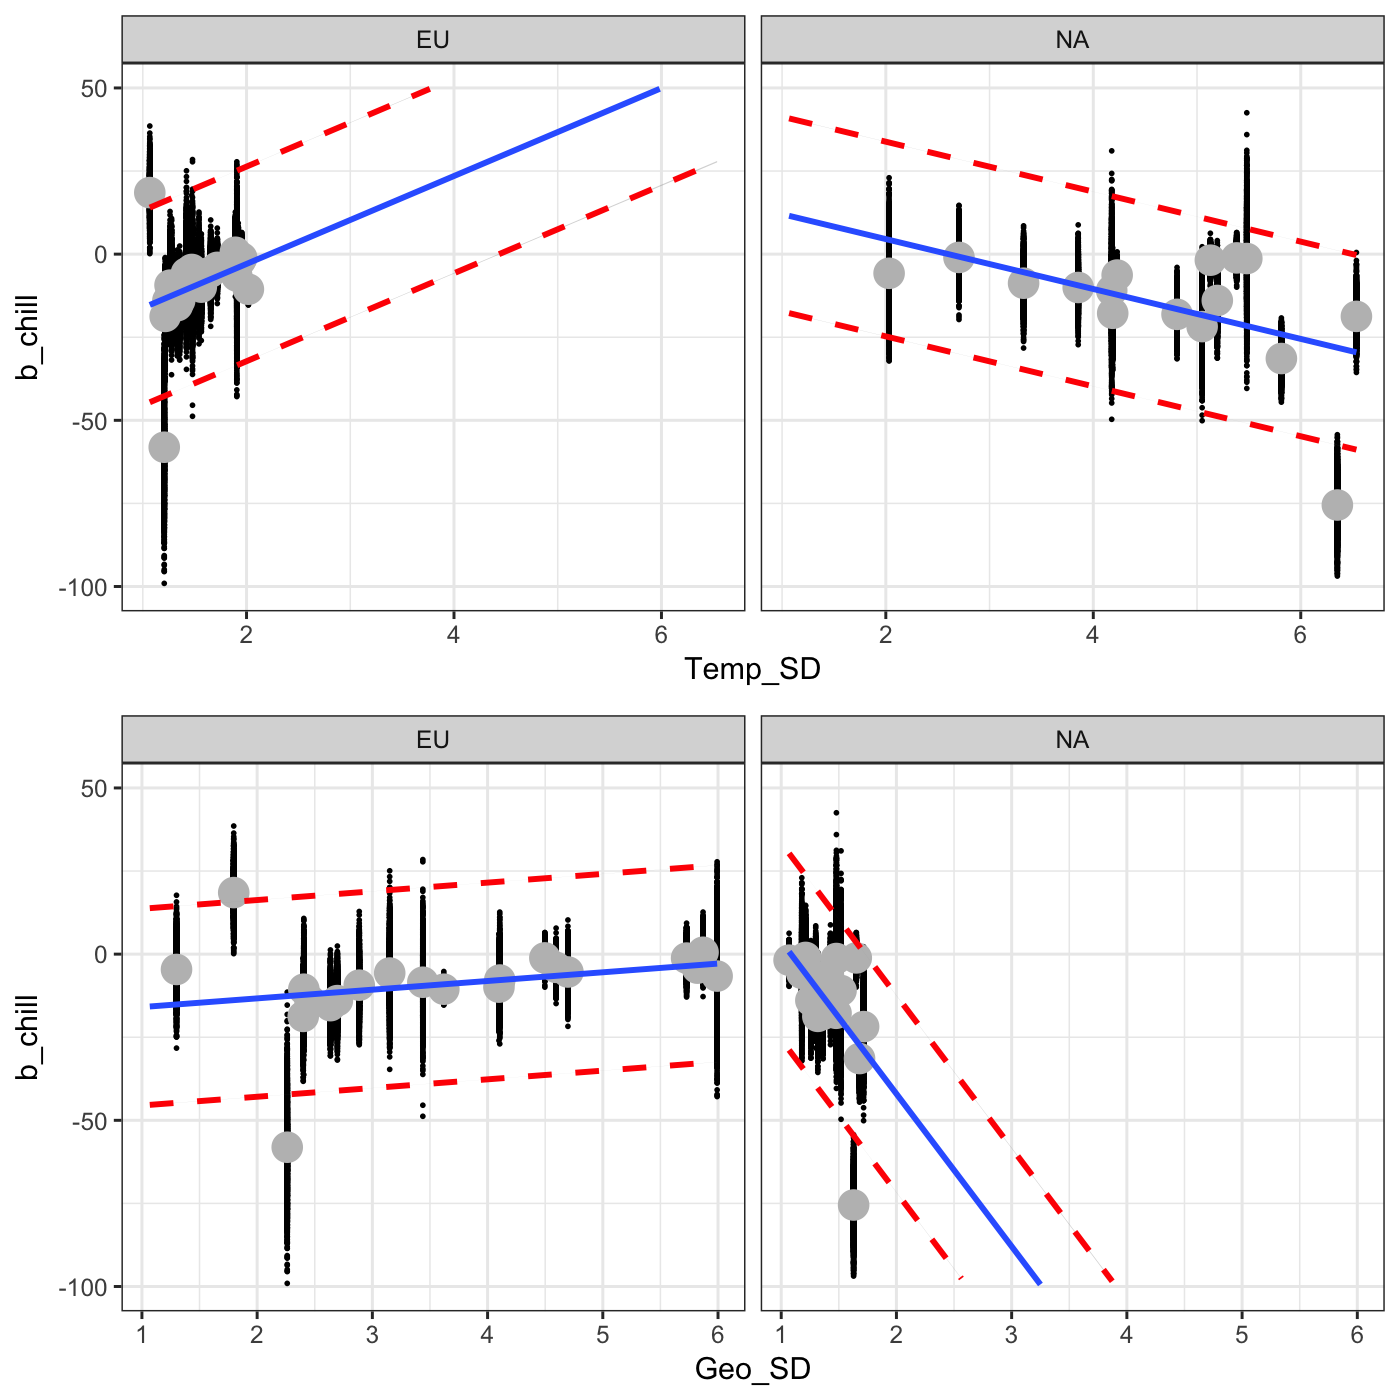
\includegraphics[width=.9\textwidth]{..//figures/cheap_approach/modeled_stv.png}
    \caption{Influence of temporal and geographic variation in mean low temperature (stv) on $\beta_{chill}$. Model is pooling on iterations. Blue line is mean and red lines 95\% credible intervals} 
    \label{fig:stv}
\end{figure}

\begin{figure}[h!]
    \centering
         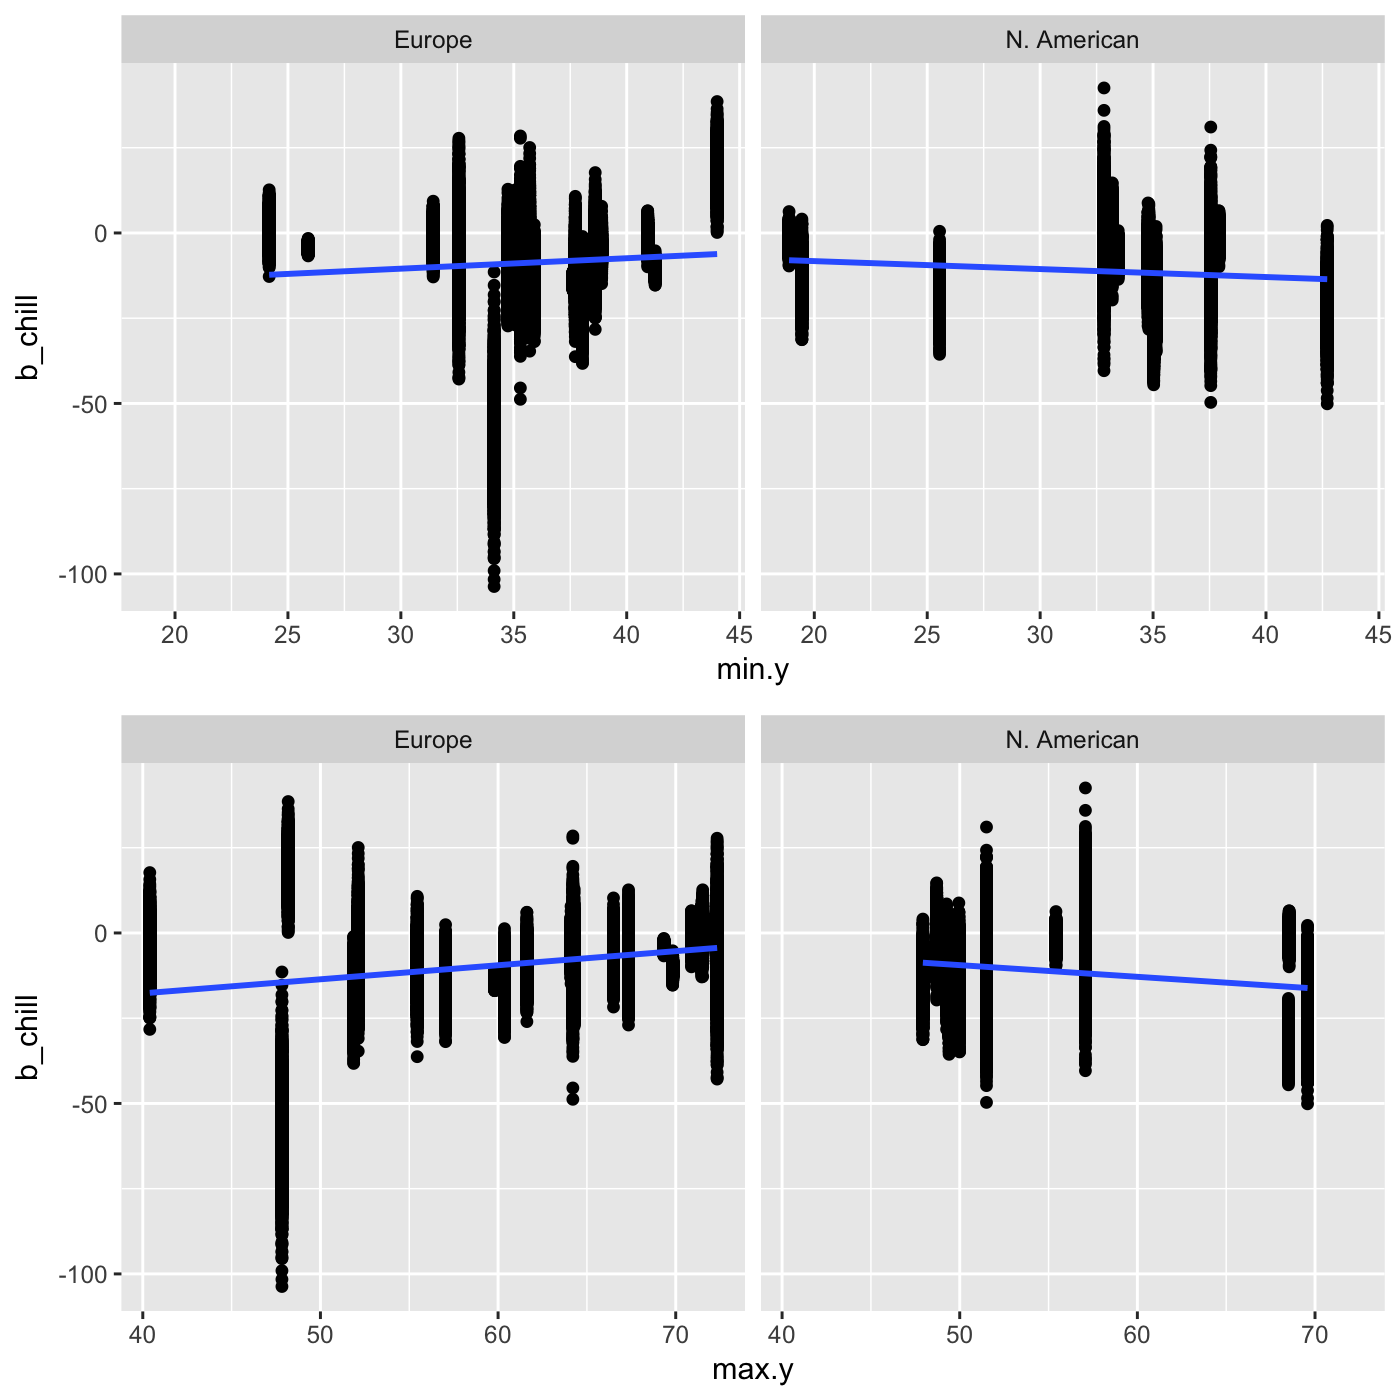
\includegraphics[width=.9\textwidth]{..//figures/cheap_approach/unmodeled_lat.png}
    \caption{Influence of max. and min latitude. on $\beta_{chill}$. No hierarchy, simple linear model for now.} 
    \label{fig:lat}
\end{figure}





\end{document}